%!TEX root = Intro-NLP-seminar.tex
\section{Example Applications of NLP}

\begin{frame}
\frametitle{Machine Translation (MT)}
\framesubtitle{e.g.~Google Translate}
\begin{itemize}
\item Automatic translation of a text from a \emph{source language} to a \emph{target language} by a computer, preserving the meaning
\item Some language pairs have good outputs; some not so good
\item \alert{(Why?)}
\framebreak
\item Analyse input $\longrightarrow$ processing $\longrightarrow$ Synthesise output
\item Need to ensure meaning is translated correctly
\item Need to ensure output is grammatically correct
\item \alert{`Translating' by dictionary look up or just translating words individually is \emph{not} MT}
\end{itemize}
\end{frame}

\plain{However\ldots}

\begin{frame}[allowframebreaks]
\frametitle{Use cases of MT}
\framesubtitle{What do you need MT for?}
\textcite[ch.~10]{Somers:2003} pointed out 3 use cases of MT.
\begin{itemize}
\item \textbf{Disemmination}
	\begin{itemize}
	\item Translation output to be distributed for human as-is without changes
	\item End users will have high expectations!
	\item Output must be more or less perfect and well-formed
	\item Hard -- except for language pairs with huge amount of training data
\framebreak
	\item Example Russian--English translation, suitable for dissemination:
		\begin{description}
		\item[Russian:] 18 февраля 2015 года Аналитическое управление аппарата Совета Федерации совместно с экономическим факультетом МГУ проводят научный семинар «Реалистическое моделирование».
		\item[English:] February 18, 2015 Analytical Department of the Federation Council in conjunction with the Faculty of Economics of Moscow State University conducted a scientific seminar ``The realistic simulation.''
		\end{description}
\framebreak
\item \textbf{Assimilation} 
	\begin{itemize}
	\item Just to get a rough idea of the content
	\item Output need not be perfect
	\item But choice of words should reflect original meaning
	% \item Example:
	% 	\begin{description}
	% 	\item[Iban:] Udah ujan nya ngetu terbubuh, matahari enggau emperaja lalu ayan ba langit
	% 	\item[English:] rain cease, sun and rainbow visible sky. 
	% 	\end{description}
	 \end{itemize}
\framebreak
	\item Example Japanese--English translation, for assimilation:
		\begin{description}
		\item[Japanese:] 世界中の優秀な頭脳を魅了し、研究に集中できるようなサポート体制の整った環境とはどのようなものでしょうか。
		\item[English:] Attracts the brightest minds in the world, what What are the well-equipped environment support system, such as can concentrate on research.
		\end{description}
	\end{itemize}
\framebreak
\item \textbf{Interchange}
	\begin{itemize}
	\item Translation in one-to-one communication (telephone or written correspondence).
	\item Internet: tweets, blog posts, forums
	\item Human translation is out of the question (too slow)!
	\item \emph{Any} output (even if poor) is better than \emph{no} output
%	\item Usually for shorter phrases and values
%	\item Context is still important to choose correct words to reflect similar meaning!
	\end{itemize}
\end{itemize}
\end{frame}

\begin{frame}
\frametitle{Some definitions}
\begin{description}[Source language]
\item[Utterance] An uninterrupted chain of spoken or written language
\item[Source language] The original language of an utterance
\item[Target language] The language the utterance to be translated to
\item[Language pair] a SL--TL pair for an MT process, in that direction
\end{description}

\end{frame}

%\againframe{MachineTranslation}

%\begin{frame}
%\frametitle{Automatic Summarisation}
%
%\end{frame}


\begin{frame}
\frametitle{Text and Corpus Processing}
    
\begin{itemize}[<+->]
\item Given a text or a corpus (a collection of documents)
\item Identify the most frequently occurring words; most significant words; group of words \ldots
\item Most frequently occuring: the, a, an\ldots probably not so important!
\item Most significant collocations ($n$-grams): finance, investment capital, tax returns\ldots\\
		$\longrightarrow$ document is probably about \textbf{Finance} or \textbf{Economy}
\item Useful for domain identification; document indexing for retrieval (search engine)
\end{itemize}

\end{frame}

\begin{frame}
\frametitle{Information Extraction (IE)} 

\begin{itemize}[<+->]
\item Extract ``interesting'' facts to store in a knowledge base 
\item `John stays in London. He works there for Polar Bear Design.'
	\begin{exampleblock}{Knowledge Base}
	$\text{John}_\text{PER} \xrightarrow{\text{live-in}} \text{London}_\text{LOC}$\\
	$\text{John}_\text{PER} \xrightarrow{\text{employee-of}} \text{Polar Bear Design}_\text{ORG}$
	\end{exampleblock}
\end{itemize}
\end{frame}


\begin{frame}
\frametitle{Another IE Example (Easier?)}
    
\begin{figure}
\centering
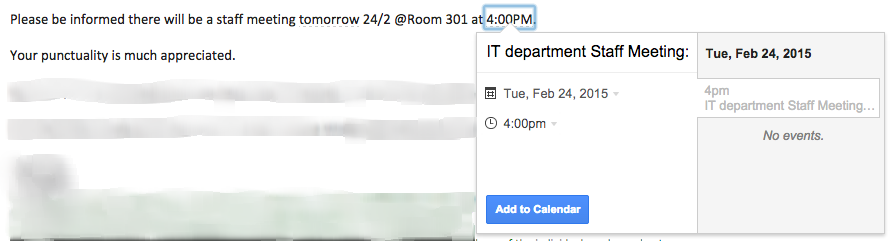
\includegraphics[width=\textwidth]{IE-event}
\end{figure}

NLP applications are often easier to design and implement with a specific use case scenario in mind

\end{frame}


\begin{frame}
\frametitle{Named Entity Recognition (NER)}

\begin{itemize}
\item Identification of proper nouns in the text
\item And classify them into catogeries of interest
\pause
\item (Typically Person, Location, Organisation, Date, Currency\ldots)
\pause
\item `\textbf{John}$_\text{PER}$ stays in \textbf{London}$_\text{LOC}$. He works there for \textbf{Polar Bear Design}$_\text{ORG}$.'
\end{itemize}

\end{frame}


\begin{frame}
\frametitle{Co-reference Resolution}

\begin{itemize}[<+->]
\item Tracking references to NEs
\item 
\tikz[baseline,remember picture]\node[anchor=base,inner sep=0pt] (john) {John}; 
stays in \tikz[baseline,remember picture]\node[anchor=base,inner sep=0pt] (london) {London};. 
\tikz[baseline,remember picture]\node[anchor=base,inner sep=0pt] (he) {He}; 
works \tikz[baseline,remember picture]\node[anchor=base,inner sep=0pt] (there) {there}; 
for Polar Bear Design. 
\tikz[overlay,remember picture]\path(he.south) edge[bend left,->,draw, >=latex'] (john.south) (there.north) edge[bend right,->,draw, >=latex'] (london.north);
\end{itemize}

\end{frame}


\begin{frame}
\frametitle{Question Answering (QA)}
\framesubtitle{e.g.~Siri}

\begin{itemize}[<+->]
\item Need to compile, index, extract a knowledge base of facts (re IE)
\item Need to analyse and interpret question to identify elements
\item Need to search knowledge base
\item May need to make inferences
\item Need to present answers in a sensible manner
\end{itemize}

\begin{columns}[T]
\begin{column}{.35\linewidth}
\begin{description}[Q:]
\item[Q:] `Where is Polar Bear Design located?'
\item[A:] London
\end{description}
\end{column}

\pause

\begin{column}{.64\linewidth}
\begin{exampleblock}{Knowledge Base}
	$\text{John}_\text{PER} \xrightarrow{\text{live-in}} \text{London}_\text{LOC}$\\
	$\text{John}_\text{PER} \xrightarrow{\text{employee-of}} \text{Polar Bear Design}_\text{ORG}$\\
	\alert{$\text{Polar Bear Design}_\text{ORG} \xrightarrow{\text{based-in}} \text{London}_\text{LOC}$}
\end{exampleblock}
\end{column}
\end{columns}

\end{frame}


\begin{frame}[allowframebreaks]
\frametitle{Plagiarism and Paraphrase Detection}
    
\begin{itemize}[<+->]
\item TurnItIn currently just detects plagiarism based on string matching
\item What about paraphrasing? Also a form of plagiarism
\item Check if several news reports are about the same event/issue
\item \parencite{li2006sentence,pera2011simpad}
\end{itemize}
\end{frame}


\begin{frame}
\frametitle{Checking the Semantic Similarity}

\url{http://swoogle.umbc.edu/StsService/GetStsSim}

\begin{itemize}
\item Inputs:
	\begin{itemize}
		\item `Many \textbf<2->{dairy} farmers today use \textbf<2->{machines} for \textbf<2->{operations} from milking to \textbf<2->{culturing} cheese.'
		\item `Today many \textbf<2->{cow} farmers perform different \textbf<2->{tasks} from milking to making \textbf<2->{cheese} using \textbf<2->{automated devices}.' 
	\end{itemize}
\item<3-> Word order, word substitutions
\item<4-> $ > 70\%$ similarity!
\end{itemize}

\end{frame}


\begin{frame}
\frametitle{Sentiment Analysis \& Opinion Mining}

\begin{itemize}
\item<1> Extract human judgement, evaluation, emotion, polarity from an utterance.
\item<1> Blogs, forum posts, tweets, speeches\ldots
\item<2> Sentimen Classfication: \url{http://text-processing.com/demo/sentiment/}
	\begin{itemize}
	\item `This movie is overrated -- all special effects, no heart.' 
		\begin{description}
			\item[Polarity] pos: 0.4; neg: 0.6 (more negative than positive)
			\item[Subjectivity] neutral: 0.2; polar: 0.8 (more subjective than objective) 
		\end{description}
	\item Negation: `It's not bad.' ???
	\end{itemize}
\item<3> More targeted:
	\begin{itemize}
	\item `The price is rather high, but the material is quite sturdy.'
	\item \texttt{[price]} -ve; \texttt{[material]} +ve
	\end{itemize}
\end{itemize}

\end{frame}

\begin{frame}
\frametitle{US 2012 Presidential Election Campaign}
    
\begin{itemize}
\item \citetitle{wang2012system} \parencite{wang2012system}
\item Twitter index tracks sentiment on Obama, Romney \href{http://usatoday30.usatoday.com/news/politics/story/2012-08-01/twitter-political-index/56649678/1}{\beamergotobutton{Link}}
\item How Social Media Sentiment Impacts the Presidential Campaigns \href{http://contently.com/strategist/2012/10/24/social-media-sentiment-becomes-factor-in-presidential-campaigns/}{\beamergotobutton{Link}}
\item Tracking sentiments of a speech \href{http://sentiment.dev.ber.to/}{\beamergotobutton{Link}}
\end{itemize}

\end{frame}


\begin{frame}
\frametitle{Speech Recognition and Synthesis}

\begin{itemize}[<+->]
\item Speech recognition: speech-to-text (STT)
	\begin{itemize}
	\item Accents, non-native speakers, pauses, filler noises\ldots
	\end{itemize}
\item Speech synthesis: text-to-speech (TTS)
	\begin{itemize}
	\item Easier? (bank teller systems etc)
	\item How to simulate \alert{natural sounding} speech?
	\end{itemize}
\end{itemize}

\end{frame}

\begin{frame}
\frametitle{Speech Recognition $\neq$ Voice Recognition}
\begin{itemize}[<+->]
\item Speech recognition
	\begin{itemize}
	\item Given a speech sample, what was said? `Dubai' or `Good bye'?
	\item Involves language modelling (statistical model of valid sentences)
	\end{itemize}
\item Voice recognition
	\begin{itemize}
	\item Given a speech sample, determine the identity of speaker
	\item Involves signal processing, voice signatures
	\end{itemize}
\end{itemize}
\end{frame}

\begin{frame}
\frametitle{Two Approaches} 
\begin{itemize}
\item Signal processing $\longrightarrow$ identify phonemes (sound units)
\item Language modelling $\longrightarrow$ likelihood of utterance
	\begin{itemize}
	\item `It's fun to recognize speech' or
	\item `It's fun to wreck a nice beach'
	\end{itemize}
\end{itemize}
\end{frame}